\chapter{Results}

\section{Query Performance}
From the data gathered for the performance of the queries plotted in Figure~\ref{fig:performance} it can be shown that even with 256 bit codes we see sub-linear query times for the larger datasets. It is also evident that these speedups are more pronounced with larger database sizes. The observed empirical optimal values of $m$ are close to but do not completely agree with the equation $b / \textrm{log}_2 n$ proposed in~\cite{norouzi2012fast}.

\begin{center}
\begin{tabular}{| l | r | r | r |}
\hline
\bfseries Dataset & \bfseries Descriptors & \bfseries Calculated Optimal $m$ & \bfseries Empirical Optimal $m$\\ \hline
MIRFLICKR-25000 & 10818284 & 10.96 & 10 \\ \hline
256 Object Category & 9996971 & 11.01 & 11  \\ \hline
102 Category Flower & 3615406 & 11.75 & 14 \\ \hline

\end{tabular}
\end{center}

\begin{figure}[H]
\figfont
\centering
\plottestIII{test3/mirflickr.final.csv}{Query time per descriptor for MIRFLICKR-25000}{398}\\
\plottestIII{test3/categories.final.csv}{Query time per descriptor for 256 Categories}{463}\\
\plottestIII{test3/102flowers.final.csv}{Query time per descriptor for 102 Flowers}{499}
\captionsetup{width=10cm}
\caption{Query time per descriptor \emph{vs} $k$ for various $m$, for each of the three vision corpora used.}
\label{fig:performance}
\end{figure}

\section{Code Distribution}

From the data gathered for the distribution of binary codes plotted in Figure~\ref{fig:bitdist} we can see that the bits are not uniformly distributed as there are almost no bits which passed a $\chi^2$ test against a uniform distribution for $p=0.05$ (bits that passed are marked in green). The assumption of uniformly distributed codes is made when calculating the theoretical performance of the MIH structure. We can also see that there is a pattern in the expected values of the bits between the 3 different datasets.


\begin{figure}[H]
\figfont
\centering
% \plottestV{test5/mirflickr.dist}{Distribution of codes for MIRFLICKR-25000}{0.499702}{0.510298}\\
% \plottestV{test5/catagories.dist}{Distribution of codes for 256 Categories}{0.48}{0.52}\\
% \plottestV{test5/102flowers.dist}{Distribution of codes for 102 Flowers}{0.4099702}{0.5900298}
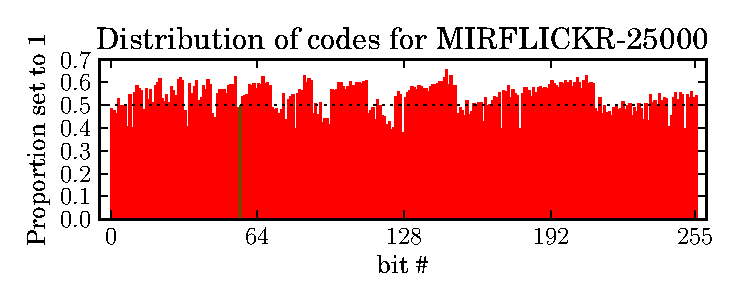
\includegraphics{test5/mirflickr.pdf}
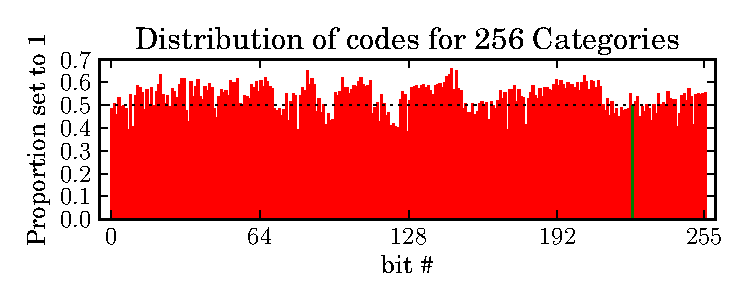
\includegraphics{test5/catagories.pdf}
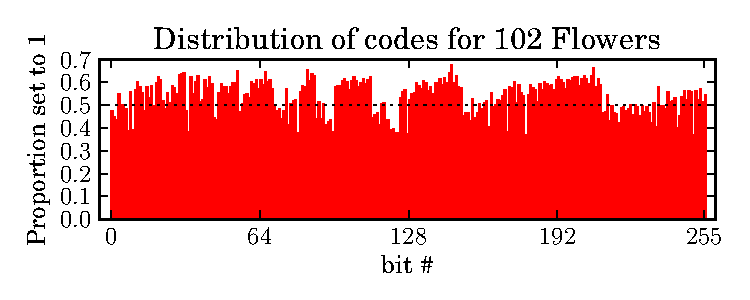
\includegraphics{test5/102flowers.pdf}
\captionsetup{width=10cm}
\caption{Empirical expected value for each bit for all codes in each of the three vision corpora used.}
\label{fig:bitdist}
\end{figure}

Text below distribution

\section{Hamming Radii needed for k-NN}

We can see from the Hamming radii required for $k=10$ and $k=1000$ nearest neighbours for our three datasets that the requred radii are much larger in our 256 bit codes compared to the 64 and 128 bit codes in Figure \ref{fig:radii}. The deviation of the required radii are also much higher for our natively generated 256 bit codes.

\begin{figure}[H]
\figfont
 
\centering
\plottestIV{test4/k10_mirflickr.radii}{MIRFLICKR-25000}{10}
\plottestIV{test4/k10_catagories.radii}{256 Categories}{10}
\plottestIV{test4/k10_102flowers.radii}{102 Flower Categories}{10}
\plottestIV{test4/k1000_mirflickr.radii}{}{1000}
\plottestIV{test4/k1000_catagories.radii}{}{1000}
\plottestIV{test4/k1000_102flowers.radii}{}{1000}
\caption{Shown are the histograms of the search radii that are required to find 10-NN and 1000-NN for 256 bit codes generated using ORB from the three datasets used.}
\label{fig:radii256}
\end{figure}

\begin{figure}[H]
\centering
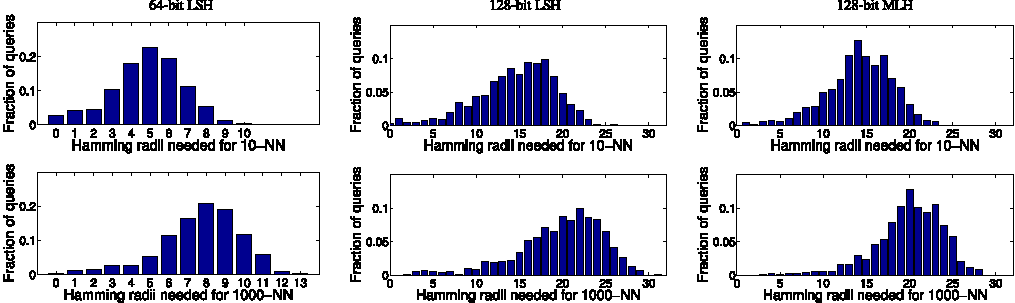
\includegraphics[width=1\textwidth]{radii64-128.pdf} 
\caption{From Norouzi \emph{et al.}~\cite{norouzi2012fast}: Shown are histograms  of the search radii that are required to find 10-NN and 1000-NN, for 64 and 128-bit code from LSH~\cite{andoni2006near}, and 128-bit codes from MLH~\cite{norouzi2011minimal}, based on 1B SIFT descriptors ~\cite{jegou2011searching}. Clearly shown are the relatively large search radii required for both the 10-NN and the 1000-NN tasks, as well as the increase in the radii required when using 128 bits versus 64 bits.
}
\label{fig:radii}
\end{figure}


\begin{figure}[p]
\figfont
\centering
\captionsetup{width=10cm}
\caption{From Norouzi \emph{et al.}~\cite{norouzi2012fast}: Recall rates for BIGANN dataset ~\cite{jegou2011searching} (1M and 1B sub-sets) obtained by K-NN on 64- and 128-bit MLH and LSH codes.}
\label{fig:hashmatching}
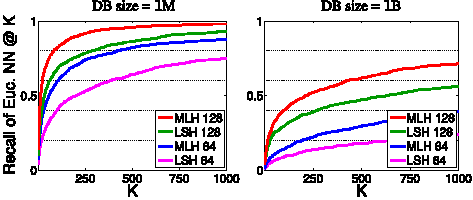
\includegraphics[width=0.5\textwidth]{LSH-MLH.pdf}
\end{figure}